%!TEX root = theory.tex
%
% =========================================================================
% -------------------------------------------------------------------------
% Transport (Advection - Dispersion):
% -------------------------------------------
%
%  This is a good place to outline key objectives of this section.
%
% -------------------------------------------------------------------------

\section{Transport Processes}    
\label{sec:transport-processes}

\subsection{Overview}

Transport is one of the most important process that needs to be accurately 
captured in the Environmental Management modeling tool set.  
In what follows, we use "Transport" to refer to the set of physical processes 
that lead to movement of dissolved and solid contaminants in the subsurface, 
treating the chemical reactions that can affect the transport 
rate through a retardation effect as a separate set of processes.  
The principal transport processes to be considered are 
\emph{advection}, \emph{mechanical dispersion}, and \emph{molecular diffusion}.  
The equation for mass conservation of species $C$ can be written as
$$\label{eq:concervation of mass general}
  \frac{\partial ( \phi \sum_\alpha [s_{\alpha} C_{\alpha,i}] )}{\partial t } +
  \bnabla \cdot \bJ_{\text{adv}} \eq \bnabla \cdot \bJ_{\text{disp}} + \bnabla \cdot \bJ_{\text{diff}} + Q,
$$
where $C_{\alpha,i}$ is concentration of $i$th species in phase $\alpha$, 
$\bJ_{\text{adv}}$ is advective flux, $\bJ_{\text{disp}}$ is the dispersive flux, 
$\bJ_{\text{diff}}$ is the diffusive flux (often grouped with the dispersive flux), and  
$Q$ is the summation of various source terms which may include reactions.
%When using Richards equations we assume that the gas phase is not moving ... 


The principal assumptions associated with the transport process models derive 
from the continuum treatment of the porous medium.  
Pore scale processes, including the resolution of variations in transport rates 
within individual pores or pore networks \citep{li2008scale,kang2006lattice,lichtner-kang-2007}, 
are generally not resolved, although some capabilities for treating multi-scale 
effects are discussed in Section~\ref{sec:transport-single-phase-dual-porosity}.  
In general, it is assumed that within any one Representative Elementary Volume (REV) 
corresponding to a grid cell all transport rates are the same.  
It will be possible, however, to define overlapping continua with distinct transport 
rates, as in the case where the fracture network and rock matrix are represented as separate continua.

Transport processes may be tightly coupled to both flow and reaction processes.  
In the case of flow, one important coupling is associated with the transport of chemical 
constituents that affect the density of the solution, which in turn affects flow rates through buoyancy.
In the case of chemical reactions, the coupling effect is normally very strong for reactive constituents.  
Chemical reactions may consume components present in the gaseous phase (e.g., CO$_2$ or O$_2$), thus 
modifying the saturation of the phase itself.  
Reactions can strongly modify gradients, and thus transport rates, by either consuming 
or producing various chemical species.

\begin{center}
\begin{longtable}{cp{7cm}c}
\caption{List of local variables.} \label{table:flow-list-of-variables} \\

\multicolumn{1}{c}{Symbol} & \multicolumn{1}{c}{Meaning} & \multicolumn{1}{c}{Units} \\
\hline  \hline 
\endfirsthead

\multicolumn{3}{c}{{\tablename} \thetable{} -- Continued} \\
\multicolumn{1}{c}{Symbol} & \multicolumn{1}{c}{Meaning} & \multicolumn{1}{c}{Units} \\
\hline  \hline 
\endhead

\hline \multicolumn{3}{c}{{Continued on next page}} \\ 
\hline \hline 
\endfoot

\hline \hline
\endlastfoot

$p_l$      & liquid pressure      &  $\upa$ \\
$\bq$      & Darcy velocity       &  $\um\ucdot\us^{-1}$  \\
$s_l$      & liquid saturation    &  $-$ \\
$\mu_l$    & liquid viscosity     &  $\upa\ucdot\us$ \\
$\rho_l$   & liquid density       &  $\ukg\ucdot\um^{-3}$ \\
$\phi$     & porosity             &  $-$  \\
$\phi_f$   & porosity of fracture &  $-$  \\
$\phi_m$   & porosity of matrix   &  $-$  \\
$\eta_l$   & molar liquid density &  $\umol\ucdot\um^{-3}$ \\
$C_i$      & concentration of $i$th species    &  $\umol\ucdot\um^{-3}$ \\


\end{longtable}
\end{center}


%%%%%%%%%%%%%%%%%%%%%%%%%%%%%%%%%%%%%%%%%%%%%%%%%%%%%%%%%%%%%%%%%%%%%%%%%%%%%%%%%%%%
%%%%%%%%%%%%%%%%%%%%%%%%%%%%%%%%%%%%%%%%%%%%%%%%%%%%%%%%%%%%%%%%%%%%%%%%%%%%%%%%%%%%
\subsection{Single-Phase Transport} 
\label{sec:transport-single-phase}

The name of this section single-phase transport indicates that we consider only one liquid phase 
(vs. multiple liquid phases).
At the same time we still consider the gas and solid phases as well.

%%%%%%%%%%%%%%%%%%%%%%%%%%%%%%%%%%%%%%%%%%%%%%%%%%%%%%%%%%%%%%%%%%%%%%%%%%%%%%%%%%%%
\subsubsection{Process Model Equations} 

The contaminants can be transported through one of three phases:
solid, liquid or gas.
When the contaminant $i$ is present in the solid phase (e.g. ice)
it is assumed not to be moving.
One of the key assumptions of Richards equations used for flow models 
is that the gas phase is not moving.  
%The transport in Amanzi neglects concentration of species in gaseous phase.
Therefore, the concervation of mass equation in its general form 
\eqref{eq:concervation of mass general}
can be separated into equations
for the liquid and gas phases.
The equation for the species $i$ dissolved in the liquid phase is
\begin{equation}  \label{eq:MassConservation}
  \frac{\partial ( \phi s_l C_{l,i} )}{\partial t } + \bnabla \cdot \bJ_{l,i}^\text{adv} 
  \eq 
  \bnabla \cdot \bJ_{l,i}^\text{disp} + \bnabla \cdot \bJ_{l,i}^\text{diff} + Q_{l,i}
\end{equation}
and the equation for the pecies $i$ in the gas phase is
\begin{equation}  \label{eq:MassConservation gas}
  \frac{\partial ( \phi s_g C_{g,i} )}{\partial t } 
  \eq 
  \bnabla \cdot \bJ_{g,i}^\text{diff} + Q_{g,i}.
\end{equation}
The gas and liquid phases are related through an equation for saturations $s_l$ and $s_g$
$$
  s_g = 1-s_l.
$$
The transition of the polutants between phases can be modeled through the source terms $Q_*$. 



%%%%%%%%%%%%%%%%%%%%%%%%%%%%%%%%%%%%%%%%%%%%%%%%%%%%%%%%%%%%%%%%%%%%%%%%%%%%%%%%%%%%
\subsubsection{Assumptions and Applicability}

We consider pure advection process and exclude the attenuation mechanisms and microbial 
behaviors that are discussed elsewhere. 
Note that there are situations where the advection could be modified by attributes of 
the transported mass and the pore structure.  
One is the potential for nonreactive anions to be repulsed by negatively charged 
solid surfaces into the center of pore throats where the velocity is faster.  
Another is the advection of inorganic and organic colloids, and microorganisms, 
whose movement can be affected by the geometry of pore throats.  
In addition to being subject to the same physicochemical phenomena as abiotic colloids, 
microorganisms have biological processes that can affect advection (e.g., temporal 
changes in surface properties due to changes in metabolic state; chemotaxis; predation).  


%%%%%%%%%%%%%%%%%%%%%%%%%%%%%%%%%%%%%%%%%%%%%%%%%%%%%%%%%%%%%%%%%%%%%%%%%%%%%%%%%%%%
\subsubsection{Advective Transport}  
\label{sec:transport-advection}

Advection is the process where the bulk fluid motion transports mass and heat.  
In the simplest conceptualization of advection, the mass of a component in a fluid 
parcel simply moves with the velocity of the fluid parcel.  
This assumes there are no other processes (e.g., diffusion, dispersion, reactions) 
that can affect the component concentration in the fluid parcel.  
Thus, advection can be a particulate or a dissolved species moving with the pore-water 
whose velocity is governed by the flow processes (discussed elsewhere).  
Continuum models have addressed these behaviors using bulk parameterizations 
to characterize the pore-scale controls and controlling chemical gradients.

Numerical difficulties with the accuracy, robustness, and computation efficiency 
of modeling the advection of moving steep concentration fronts, especially in 
complex velocity fields, are well known.  
In some cases, there are constraints on the Peclet and Courant numbers for the 
useful application of a given technique.
The advective flux, $\bJ_{\text{adv}}$, of a dissolved species is described 
mathematically as
\begin{equation} \label{eq:AdvectiveFlux} 
  \bJ_{l,i}^\text{adv} = \phi s_l \bv_l C_{l,i},  
\end{equation}
where $\phi$ is the porosity, $s_l$ is liquid saturation, $\bv_l$ is the 
average linear velocity of the liquid, and $C_{l,i}$ is the concentration of the $i$th species in the liquid phase.


%%%%%%%%%%%%%%%%%%%%%%%%%%%%%%%%%%%%%%%%%%%%%%%%%%%%%%%%%%%%%%%%%%%%%%%%%%%%%%%%%%%%
\subsubsection{Dispersive Transport}   
\label{sec:transport-dispersion}

\subsubsection{Overview}

Dispersion of a dissolved constituent refers to its spreading along tortuous pathways in a porous medium caused by mixing effects.  
Dispersion takes place in the direction of the flow (longitudinal) and normal to the flow (transverse).  
A conventional Eulerian Fickian representation of dispersion is assumed, 
which may be taken as the asymptotic limiting form of the dispersion tensor \citep{neuman1990universal}. 
It should be noted that issues related to the scale dependence of dispersion are not considered.  
While this approach is known to have several limitations, 
such as backward dispersion against the direction of flow and scale independence, nevertheless, 
it is still widely used in practical applications. 
Furthermore, it may be the only approach for representing local scale dispersion. 

\subsubsection{Process Model Equations}

The dispersive flux $\bJ_i^{\rm disp}$ for a variably saturated porous medium has the form
\EQ
  \bJ_i^{\rm disp} \eq -\phi s_\a \bD\bnabla C_i,
\EN
described in analogy to a Fickian process, where $\bD$ denotes the dispersion tensor.
The dispersion tensor takes different forms depending on whether the media is isotropic or anisotropic.


\paragraph{Isotropic Media.}
For an isotropic medium with no preferred axis of symmetry the dispersion tensor $\bD^{}$ has the well-known form \citep{bear-1972}
\BA\label{isotropic}
\renewcommand{\arraystretch}{2}
\bD^{} &\eq \a_T v \bI + \left(\a_L-\a_T \right)\frac{\bv\bv}{v},\\
&\eq \left(
\begin{array}{ccc}
\a_T v + (\a_L-\a_T)\dfrac{v_x^2}{v} & (\a_L-\a_T)\dfrac{v_x v_y}{v} & (\a_L-\a_T)\dfrac{v_x v_z}{v}\\
(\a_L-\a_T)\dfrac{v_y v_x}{v} & \a_T v + (\a_L-\a_T)\dfrac{v_y^2}{v} & (\a_L-\a_T)\dfrac{v_y v_z}{v}\\
(\a_L-\a_T)\dfrac{v_z v_x}{v} & (\a_L-\a_T)\dfrac{v_z v_y}{v} & \a_T v + (\a_L-\a_T) \dfrac{v_z^2}{v}
\end{array}
\right),
\EA
characterized by the two parameters $\a_L$ [m] and $\a_T$ [m] referred to the longitudinal and transverse dispersivity, respectively. The vector $\bv = (v_x,\,v_y,\,v_z)$ [m/s] denotes the average pore velocity with magnitude $v$, and $\bI$ is the identity matrix.  

\paragraph{Anisotropic Media.}

The dispersion tensor for anisotropic media has not received much attention,  However, it has been shown that in an axi-symmetric medium with axis of symmetry $\blambda_s$, the dispersion tensor takes the general form \citep{lichtner_2002}
\BA     \label{gendisp}
\bD^{} \eq \a_T^H v \bI &+ \left[ \a_L^H-\a_T^V + \cos^2\!\theta \left( \a_L^V-\a_L^H+\a_T^V-\a_T^H \right) \right] \frac{\bv\bv}{v} \nonumber\\
& + \left(\a_T^V-\a_T^H \right) v \left[ \blambda_s\blambda_s - \dfrac{\cos\theta}{v} \left(\blambda_s\bv+\bv\blambda_s \right) \right],
\EA
where $\a_L^{H,\,V}$ and $\a_T^{H,\,V}$ refer to the longitudinal and transverse dispersivity in the horizontal and vertical directions, and $\theta$ denotes the angle between the axis of symmetry and the flow velocity.




%%%%%%%%%%%%%%%%%%%%%%%%%%%%%%%%%%%%%%%%%%%%%%%%%%%%%%%%%%%%%%%%%%%%%%%%%%%%%%%%%%%%
\subsubsection{Diffusive Transport} 
\label{sec:transport-diffusion}



\subsubsection{Overview}

\noindent Molecular diffusion is often indistinguishable from mechanical dispersion as a process operating in porous media, and thus the two are often lumped together to form a hydrodynamic dispersion term.  Unlike dispersion, however, there is no effect of flow direction, so the potential difficulties associated with mismatches between flow and grid coordinate direction do not arise.  Molecular diffusion is an entropy-producing process in which the random motion of molecules causes spreading or homogenization of a concentration field.  Atomistic representations of molecular diffusion capture this random motion, but continuum models of the kind considered here typically represent only the average behavior of the molecules.  It is noteworthy, however, that atomistic and continuum models for molecular diffusion do agree if sufficiently long time scales with a sufficient number of molecules are considered \citep{bourg2008modeling}.

\noindent The principal distinctions in the treatment of molecular diffusion are between those based on Fick's Law, which states that the diffusive flux is linearly proportional to the concentration gradient, and multicomponent treatments that take into account the buildup of electrostatic forces as the individual charged species (ions) attempt to diffuse at their own rate.  In addition, a full treatment of molecular diffusion involves calculating fluxes in terms of gradients in chemical potential rather than concentration \citep{steefel2009fluid}.

\noindent In addition to the complexities associated with chemical interactions, it is also necessary to account for the effects of the porous medium through which diffusion occurs.  Corrections to the diffusive flux are often represented with a tortuosity (see Section~\ref{sec:tortuosity} below) based on an upscaled constitutive law intended to capture the heterogeneous pore geometries.  Since diffusion may be restricted or eliminated through narrow pore throats, the effective diffusivity for a specific ion may be quite different from its diffusivity in water alone.  Capturing the multiscale nature of the pore structure and its effect on molecular diffusion remains a challenge.



\subsubsection{Process Model Equations}

\paragraph{General Formulation for Molecular Diffusion.}

The most rigorous and general expression for molecular diffusion is given by
\begin{equation} \label{eq:OnsagerReciprocal} 
  \boldsymbol{J}_{j}^{\rm diff} =-\sum_{i}{L_{ji}\boldsymbol{\nabla}\frac{\mu _{i}}{T}},
\end{equation} 
where the $L_{ji}$ are the phenomenological coefficients introduced in
the theory of irreversible thermodynamics
\citep{onsager1931reciprocal,prigogine1968introduction,lasaga1998kinetic}
and $\mu_j$ is the chemical potential of the $i$th species.  Here, the
fluxes are linearly related to gradients in the chemical potentials of
the solutes rather than to their concentrations as in Fick's Law that
follows.  The phenomenological coefficients, $L_{ji}$, can be linked
back to measurable quantities by making use of the mobility as the
``velocity'' of a particle acted upon by a force, with the force in
this case provided by the chemical potential rather than the
concentration
\begin{equation} \label{eq:ChemicalPotentialGradient)} 
  \boldsymbol{J}_{j}^{\rm diff} =-\boldsymbol{\nabla} ( u_{j} C_{j} \mu _{j}), 
\end{equation} 
where $u_{j}$ is the mobility of the $j$th ion defined by
\begin{equation} \label{eq:IonMobility} 
  u_{j} \eq \frac{D_j}{RT}.
\end{equation} 



\paragraph{Single Species Diffusion (Fick's Law).}

Molecular diffusion is usually described in terms of Fick's First Law, which states that the diffusive flux is proportional to the concentration gradient
\begin{equation} \label{eq:FicksFirstLaw} 
\boldsymbol{J}_{i}^\text{diff} \eq -\boldsymbol{\nabla} \left( D_{i} C_{i} \right).  
\end{equation} 
$D_i$ is referred to as the diffusion coefficient and is specific to the chemical component considered as indicated by the subscript $i$.  Fick's First Law is a phenomenological theory for diffusion that relates diffusion to the ``driving force'' provided by the concentration gradient, although it can also be derived atomistically \citep{lasaga1998kinetic}.   In the case of diffusion in porous media, it is normally necessary to include a tortuosity correction as well (see discussion below).  

\paragraph{Tortuosity.}\label{sec:tortuosity}
Since water-rock interaction commonly takes place in porous materials, 
it is important to account for the effect of tortuosity (Figure ~\ref{fig:Tortuosity}), 
which is defined as the ratio of the path length the solute would follow in water alone, $L$, 
relative to the tortuous path length it would follow in porous media, $L_e$ \citep{bear-1972}
\begin{equation} \label{eq:Tortuosity} 
  \tau_{L} 
  =
  \left({\raise0.7ex\hbox{$ L $}\!\mathord{\left/ {\vphantom {L L_{e} }} \right. 
  \kern-\nulldelimiterspace}\!\lower0.7ex\hbox{$ L_{e}  $}} \right)^{2}.  
\end{equation} 
In this definition of tortuosity (sometimes the inverse of Equation \eqref{eq:Tortuosity} is used), 
its value is always less than one and the effective diffusion coefficient in porous media 
is obtained by multiplying the tortuosity by the diffusion coefficient for the solute in pure water. 
\begin{figure}
\begin{center}
  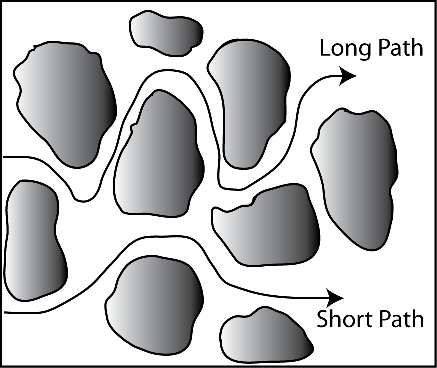
\includegraphics[scale=0.5]{figs/Figure4-Steefel.pdf}
  \caption{Tortuous diffusion paths in porous media \citep{steefel2009fluid}}
  \label{fig:Tortuosity}
\end{center}
\end{figure}

With this formulation, the diffusion coefficient in porous media, $D_{i}^{*}$, is given by
\begin{equation} \label{eq:EffectiveDiffusion)} 
  D_{i}^{*} =\tau_{L} D_{i}.  
\end{equation} 
The diffusive flux, then, is given by
\begin{equation} \label{eq:DiffusiveFluxPorousMedia)} 
  \boldsymbol{J}_{j}^{\rm diff} 
  \eq 
  -\boldsymbol{\nabla} \left( \phi s_{\alpha} D_{j} \tau_{L} C{}_{j} \right) 
  \eq 
  -\boldsymbol{\nabla} \left( \phi s_{\alpha} D_{j}^{*} C{}_{j} \right) .  
\end{equation} 
Various approaches for calculating formation factors (and thus, the diffusion coefficient in porous medium) are in use, 
with a formulation based on Archie's Law being the most common for fully saturated (single phase) systems
\begin{equation} \label{eq:CementationExponent} 
  F_f  \eq \frac{1}{a\phi ^{m} } ,  
\end{equation} 
where $a$ is a unitless fitting constant and $m$ is unitless the cementation exponent.  

For partially saturated systems, it is common to use the Millington-Quirk formulation 
\citep{millington1961permeability, sumner-handbook, moldrup2000predicting}
\begin{equation}   \label{eq:MillingtonQuirk}
  D_{i}^{*} \eq \phi^{4/3} s_{\alpha}^{10/3}  D_{i},
\end{equation}
where the saturation, $s_{\alpha}$, can refer to either the gas or the aqueous phase.







%%%%%%%%%%%%%%%%%%%%%%%%%%%%%%%%%%%%%%%%%%%%%%%%%%%%%%%%%%%%%%%%%%%%%%%%%%%%%%%%%%%%
%%%%%%%%%%%%%%%%%%%%%%%%%%%%%%%%%%%%%%%%%%%%%%%%%%%%%%%%%%%%%%%%%%%%%%%%%%%%%%%%%%%%
\subsection{Single-Phase Transport with Dual Porosity Model} 
\label{sec:transport-single-phase-dual-porosity}

The multiscale nature of porous media and the transport processes associated is 
arguably the most significant and largely unresolved challenge for simulation of 
fate and transport in subsurface aquifers.  
Transport actually operates at the pore scale where variations in flow velocity 
and reaction rates can result in microscopic variability in transport rates.  
Continuum treatments of transport in porous media cannot resolve such sub-grid 
variations easily, although various upscaling techniques may be available for 
capturing the smaller scale behavior.  
In addition, multi-continuum or hybrid approaches may obviate the need for a formal 
upscaling procedure, although there are significant computational difficulties and 
expense associated with their implementation.


%%%%%%%%%%%%%%%%%%%%%%%%%%%%%%%%%%%%%%%%%%%%%%%%%%%%%%%%%%%%%%%%%%%%%%%%%%%%%%%%%%%%
\subsubsection{Process Model Equations} 

The dual porosity formulation of the solute transport consists of two equations
for the fracture and matrix regions. 
In the fracture region, we have \citep{simunek-vangenuchten_2008}
\begin{equation}  \label{eq:MassConservation}
  \frac{\partial (\phi_f s_{lf} C_f)}{\partial t} 
  + 
  \bnabla \cdot \bJ^\text{adv} \eq \bnabla \cdot \bJ^\text{disp} 
  + 
  \bnabla \cdot \bJ^\text{diff} - \Sigma_s + Q_f,
\end{equation}
where $s_{lf}$ is liquid saturation in fracture, 
$\Sigma_s$ is the solute exchange term,
and $Q_f$ is source or sink term.
In the matrix region, we have
$$
  \frac{\partial (\phi_m s_{lm} C_m)}{\partial t}
  = \Sigma_s + Q_m,
$$
where $s_{lm}$ is liquid saturation in matrix, $Q_m$ is source or sink term.
The solute exchange term is defined as
$$
  \Sigma_s = \alpha_s (C_f - C_m) + \Sigma_w C^*,
$$
where $C^*$ is equal to $C_f$ if $\Sigma_w > 0$ and $C_m$ if $\Sigma_w < 0$.
The coefficient $\alpha_s$ is the first-order solute mass transfer coefficient [$\us^{-1}$].



%%%%%%%%%%%%%%%%%%%%%%%%%%%%%%%%%%%%%%%%%%%%%%%%%%%%%%%%%%%%%%%%%%%%%%%%%%%%%%%%%%%%
%%%%%%%%%%%%%%%%%%%%%%%%%%%%%%%%%%%%%%%%%%%%%%%%%%%%%%%%%%%%%%%%%%%%%%%%%%%%%%%%%%%%
\subsection{Boundary Conditions, Sources and Sinks} 
\label{sec:transport-boundary-conditions}

\noindent 
A number of boundary conditions are possible for the diffusive flux, 
including a Dirichlet (or first-type) boundary conditions (fixed concentration) 
and Neumann (or second-type or flux) boundary conditions. 
\todo[color=cyan]{GEH:  I suggest that we stick with third-type as the title for this boundary condition.  
It is technically Robin (definitely not Cauchy), but third-type is commonly used in subsurface reactive transport.  
I also suggest that we remove First-Type and Second-Type and simply refer to them as Dirichlet (specified concentration) and Neumann (specified flux).}

\noindent \textit{First-Type or Dirichlet Boundary Condition}:  
A first-type or Dirichlet condition involves specification of a fixed value (typically) of the concentration, $C_0$, at the boundary location,
\begin{equation} \label{eq:Dirichlet}
  \boldsymbol{C}(\boldsymbol{x})=\boldsymbol{C}_{0} .
\end{equation}

\textit{Second-Type or Neumann Boundary Condition}:  
A second-type or Neumann (or flux) boundary condition involves specification of the flux
\begin{equation}   \label{eq:Neuman}
  \boldsymbol{J}_{i}=\alpha,
\end{equation}
or concentration gradient
\begin{equation}
  \frac{\partial \boldsymbol{C}}{\partial \boldsymbol{n}} = \alpha,
\end{equation}
where $\alpha$ is a prescribed value of the flux or concentration gradient. The flux term can be a total, advective, or diffusive flux.





\subsection{Data Needs}

\noindent For modeling of molecular diffusion in porous media, two kinds of data are needed:
%
\begin{enumerate}
\item  
  Experimental data on the diffusivities of individual ions in aqueous solution;
\item  
  Characterization of the tortuosity of the porous medium under consideration.  
  The tortuosity of the medium may be determined by a number of methods, 
  including transport experiments involving tracers \citep{navarre2009evolution},
  and microscopic imaging of the porous medium using synchrotron X-ray
  %~\todo{synchrotron X-ray? -Williamson} 
  or related methods \citep{navarre2009evolution}, or estimation based on grain size and mineralogy of the materials.  
  In addition, it may be possible to determine tortuosity from effective diffusion coefficients determined in field-scale experiments.
\end{enumerate}

\noindent  
For the diffusivities of individual ions, there are some compilations in the literature \citep{lasaga1998kinetic,steefel2009fluid}.  
While the diffusivity of individual ions could in theory be calibrated from field tests, 
normally they should be determined independently so that a more accurate determination of the tortuosity can be carried out.







